\textbf{Сжатие данных} -- это процесс, обеспечивающий уменьшение объема данных путем сокращения их избыточности.
\begin{flushright}
  К. Шеннон
\end{flushright}
\parКлода Шеннона принято считать основоположником науки о сжатии информации. Его теорема об оптимальном кодировании показывает, к чему нужно стремиться при кодировании информации и насколько та или иная информация при этом сожмется. Кроме того, им были проведены опыты по эмпирической оценке избыточности английского текста. Шенон предлагал людям угадывать следующую букву и оценивал вероятность правильного угадывания. На основе ряда опытов он пришел к выводу, что количество информации в английском тексте колеблется в пределах 0,6 – 1,3 бита на символ. Несмотря на то, что результаты исследований Шеннона были по--настоящему востребованы лишь десятилетия спустя, трудно переоценить их значение.\\
\\\emph{Сжатие данных} -- это частный случай \emph{кодирования} данных и важнейший аспект передачи данных, который дает возможность более оперативно передавать данные. 
\\\\\emph{Цель сжатия} -- уменьшение количества бит, необходимых для хранения или передачи заданной информации. Это дает возможность передавать сообщения более быстро и хранить более экономно и оперативно (последнее означает, что операция извлечения данной информации с устройства ее хранения будет проходить быстрее, что возможно, если скорость распаковки данных выше скорости считывания данных с носителя информации).\\
\\Сжатие позволяет, например, записать больше информации на дискету, "увеличить" размер жесткого диска, ускорить работу с модемом и т.д. При работе с компьютерами широко используются программы--архиваторы данных формата ZIP, GZ, ARJ и других. Методы сжатия информации были разработаны как математическая теория, которая долгое время (до первой половины 80--х годов), мало использовалась в компьютерах на практике.\\
\\Введем ряд определений, которые будут использоваться далее в изложении материала.
\\\textbf{Алгоритм сжатия данных (алгоритм архивации)} -- это алгоритм, который устраняет избыточность записи данных.
\\\textbf{Символ} -- наименьшая единица данных, рассматриваемая как единое целое при кодировании/декодировании.
\\\textbf{Алфавит} -- множество всех возможных символов. При сжатии англоязычных текстов обычно используют множество из 128 ASCII кодов. При сжатии изображений множество значений пиксела может содержать 2, 16, 256 или другое количество элементов.
\\
\\Рассмотрим на примере. Возьмем обычную книгу и будем считать ее содержимое как за исходные данные. За символ мы можем взять как букву (и тогда алфавитом будет являться обычный алфавит русского языка), так и целое слово (тогда алфавит будет состоять из всех уникальных слов, встречающихся в этой книге). Символ -- не обязательно один знак. Символом могут являться слова и даже целые предложения.\\
\\\textbf{Токен} -- единица данных, записываемая в сжатый поток некоторым алгоритмом сжатия. Токен состоит из нескольких полей фиксированной или переменной длины.
\\\textbf{Фраза} -- фрагмент данных, помещаемый в словарь для дальнейшего использования в сжатии.
\\\textbf{Код} -- правило соответствия набора знаков одного множества $X$ знакам другого множества $Y$.
\\\textbf{Кодирование} -- процесс преобразования символов алфавита $Х$ в символы алфавита $Y$.
\\\textbf{Декодирование} -- процесс, обратный кодированию, при котором осуществляется восстановление данных.
\\\textbf{Кодовый символ} -- наименьшая единица данных, подлежащая сжатию. Обычно символ – это 1 байт, но он может быть битом, тритом {0,1,2}, или чем--либо еще.
\\\textbf{Кодовое слово} -- это последовательность кодовых символов из алфавита кода.
\\\textbf{Средняя длина кодового слова} -- это величина, которая вычисляется как взвешенная вероятностями сумма длин всех кодовых слов.
\\То есть:
$$ L = \sum_{i=1}^{N}p_{i}\times l_{i},$$ где: 
\\$N$ -- количество кодовых слов в алфавите;
\\$p_{i}$ -- вероятность появления кодового слова в последовательности;
\\$l_{i}$ -- количество символов в кодовом слове (длина кодового слова).
\\Сумма всех $p_{i}$ должна быть равна единице.
\\
\\Если все кодовые слова имеют одинаковую длину, то код называется \textbf{равномерным} (фиксированной длины). Если встречаются слова разной длины, то -- \textbf{неравномерным} (переменной длины).
\\
\\Классический пример равномерного кода -- таблица символов ASCII. Любой символ из этой таблицы будет закодирован одним байтом (один символ всегда кодируется двумя цифрами в шестнадцатеричной системе счисления).
\\Пример неравномерного кода -- азбука Морзе.
\\
\begin{center}
  \textbf{Характеристики кодирования}
\end{center}
\begin{table}[h]
\begin{center}
\begin{tabular}{c c c}
\multirow{2}{*}{Коэффициент сжатия} & \multirow{2}{*}{ = }  & Размер входного потока  \\
\hhline{~~--}
 &  & Размер выходного потока
\end{tabular}
\end{center}
Значения больше 1 обозначают сжатие, а значения меньше 1 – расширение.
\end{table}
\begin{table}[h]
\begin{center}
\begin{tabular}{c c c}
\multirow{2}{*}{Отношение сжатия} & \multirow{2}{*}{ = }  & Размер выходного потока  \\
\hhline{~~--}
 &  & Размер входного потока
\end{tabular}
\end{center}
Значение 0,6 означает, что данные занимают 60\% от первоначального объема. Значения больше 1 означают, что выходной поток больше входного (отрицательное сжатие, или расширение).
\end{table}

Сжатие данных можно разделить на два основных типа:
\begin{itemize}
\item \textbf{Сжатие без потерь} (\emph{полностью обратимое}) -- это метод сжатия данных, при котором ранее закодированная порция данных восстанавливается после их распаковки полностью без внесения изменений. Для каждого типа данных, как правило, существуют свои оптимальные алгоритмы сжатия без потерь;
\item \textbf{Сжатие с потерями} (\emph{частично обратимое}) --  это метод сжатия данных, при котором для обеспечения максимальной степени сжатия исходного массива данных часть содержащихся в нем данных отбрасывается. Для текстовых, числовых и табличных данных использование программ, реализующих подобные методы сжатия, является неприемлемыми. В основном такие алгоритмы применяются для сжатия аудио-- и видеоданных, статических изображений.
\end{itemize}
Существуют два основных способа проведения сжатия:
\begin{itemize}
\item \textbf{Статические методы} -- методы сжатия, присваивающие коды переменной длины символам входного потока, причем более короткие коды присваиваются символам или группам символам, имеющим большую вероятность появления во входном потоке. Лучшие статистические методы применяют кодирование Хаффмана.
\item \textbf{Словарное сжатие} -- это методы сжатия, хранящие фрагменты данных в <<словаре>> (некоторая структура данных). Если строка новых данных, поступающих на вход, идентична какому--либо фрагменту, уже находящемуся в словаре, в выходной поток помещается указатель на этот фрагмент. Важно заметить, что иногда словарь может передаваться в начале самого сообщения.
\end{itemize}

\textbf{Префиксный код} -- это код, в котором никакое кодовое слово не является префиксом любого другого кодового слова. Эти коды имеют переменную длину.
\\
\\\textbf{Оптимальный префиксный код} -- это префиксный код, имеющий минимальную среднюю длину.
\\
\newpage
\section{Алгоритмы сжатия данных}
\subsection{Алгоритм Шеннона--Фано}
\begin{wrapfigure}[13]{l}{3cm}
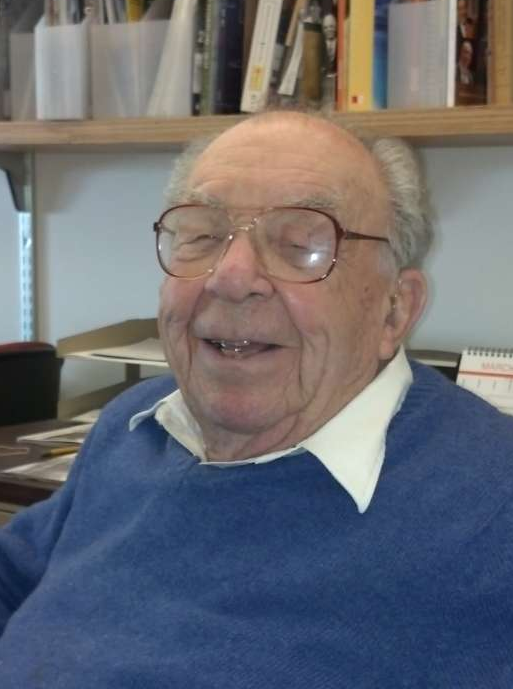
\includegraphics[width=3cm]{5_1}
\begin{center}
\caption{}
\footnotesize{Роберт Фано}
\\\footnotesize{$\mbox{род.} 1917$}
\end{center}
\end{wrapfigure}
Алгоритм Шеннона--Фано -- один из первых алгоритмов сжатия. Его сформулировали два ученых -- Клод Шеннон и Роберт Фано. Алгоритм основан на частоте повторения. Так, часто встречающийся символ кодируется кодом меньшей длины, а редко встречающийся -- кодом большей длины.
Коды, полученные при кодировании, префиксные, что позволяет декодировать любую последовательность.
\\
\\Алгоритм Шеннона--Фано для некоторых последовательностей может сформировать неоптимальные коды.
\\
\begin{center}
\textbf{Алгоритм Шеннона--Фано}
\end{center}

\begin{enumerate}
\item Символы входного (первичного) алфавита выписывают по убыванию вероятностей -- это корень будущего дерева.
\item Строится дерево от корня к листьям. Находится середина, которая делит корень на два узла. Эти узлы (суммы вероятностей символов алфавита) примерно равны.
\item Полученные узлы -- листья дерева. Левому узлу (с большей суммарной вероятностью) присваивается значение $1$, а правому -- $0$.
\item Шаги 2--3 повторяются, пока в листьях дерева не останется один символ первичного алфавита.
\item Символ входного (первичного) алфавита кодируется последовательностью нулей и единиц в соответствии с распределением их от корня к листьям (узлам).
\end{enumerate}
\emph{\textbf{Пример 1:}}
\\\emph{Задание:} составить код Шеннона--Фано для последовательности
\\$AAABCCCCCDEEEF$. Найти среднюю длину кодового слова.
\\\emph{Решение:} в последовательности AAABCCCCCDEEEF алфавит состоит из 6 символов: A, B, C, D, E, F. Выпишем символы первичного алфавита по убыванию вероятностей:
\\$\bullet$ Вероятность символа $C$ -- $^5/_{14}$;
\\$\bullet$ Вероятность символа $A$ -- $^3/_{14}$;
\\$\bullet$ Вероятность символа $E$ -- $^3/_{14}$;
\\$\bullet$ Вероятность символа $B$ -- $^1/_{14}$;
\\$\bullet$ Вероятность символа $D$ -- $^1/_{14}$;
\\$\bullet$ Вероятность символа $F$ -- $^1/_{14}$.
\\Полученная последовательность $CAEDBF$ является корнем будущего дерева.
\\Построим дерево от корня к листьям:
\begin{table}[h]
\centering
\begin{tabular}{c c c c c c}
\multicolumn{6}{c}{CAEBDF ($^5/_{14} + ^3/_{14} + ^3/_{14} + ^1/_{14} + ^1/_{14} + ^1/_{14}$)} \\
\multicolumn{2}{c}{$\downarrow$} & \multicolumn{4}{c}{$\downarrow$} \\
\multicolumn{2}{c}{CA ($^5/_{14} + ^3/_{14}$)} & \multicolumn{4}{c}{EBDF ($^3/_{14} + ^1/_{14} + ^1/_{14} + ^1/_{14}$)} \\
$\downarrow$ & $\downarrow$ & \multicolumn{2}{c}{$\downarrow$} & \multicolumn{2}{c}{$\downarrow$} \\
C ($^5/_{14}$) & A ($^3/_{14}$) & \multicolumn{2}{c}{EB ($^3/_{14} + ^1/_{14}$)} & \multicolumn{2}{c}{DF ($^1/_{14} + ^1/_{14}$)} \\
 & & $\downarrow$ & $\downarrow$ & $\downarrow$ & $\downarrow$ \\
 & & E ($^3/_{14}$) & B ($^1/_{14}$) & D ($^1/_{14}$) & F($^1/_{14}$) \\
\end{tabular}
\end{table}
\\Присвоим левому символу (с большей вероятностью) значение $1$, а правому -- $0$:
\begin{table}[h]
\centering
\begin{tabular}{c c c c c c}
\multicolumn{6}{c}{CAEBDF ($^5/_{14} + ^3/_{14} + ^3/_{14} + ^1/_{14} + ^1/_{14} + ^1/_{14}$)} \\
& $\downarrow$ & \multicolumn{4}{c}{$\downarrow$} \\
\multicolumn{2}{c}{CA ($^5/_{14} + ^3/_{14}$) [1]} & \multicolumn{4}{c}{EBDF ($^3/_{14} + ^1/_{14} + ^1/_{14} + ^1/_{14}$) [0]} \\
$\downarrow$ & $\downarrow$ & \multicolumn{2}{c}{$\downarrow$} & \multicolumn{2}{c}{$\downarrow$} \\
C ($^5/_{14}$) [1] & A ($^3/_{14}$) [0] & \multicolumn{2}{c}{EB ($^3/_{14} + ^1/_{14}$) [1]} & \multicolumn{2}{c}{DF ($^1/_{14} + ^1/_{14}$) [0]} \\
 & & $\downarrow$ & $\downarrow$ & $\downarrow$ & $\downarrow$ \\
 & & E ($^3/_{14}$) [1] & B ($^1/_{14}$) [0] & D ($^1/_{14}$) [1] & F($^1/_{14}$) [0] \\
\end{tabular}
\end{table}
\\
\\Получим следующую таблицу для кодировки:
\begin{table}[h]
\begin{tabular}{|c|c|c|}
\hline
Символ & Вероятность & Код \\
\hline
C & $^5/_{14}$ & 11 \\
A & $^3/_{14}$ & 10 \\
E & $^3/_{14}$ & 011 \\
B & $^1/_{14}$ & 010 \\
D & $^1/_{14}$ & 001 \\
F & $^1/_{14}$ & 000 \\
\hline
\end{tabular}
\end{table}
\\Исходная последовательность AAABCCCCCDEEEF кодируется следующей: $10.10.10.010.11.11.11.11.11.001.011.011.011.000 -- 34$ бита.
\\Средняя длина кодового слова: $^5/_{14}\times 2 + ^3/_{14}\times 2 + ^3/_{14}\times 3 + ^1/_{14}\times 3\hm + ^1/_{14}\hm\times 3\hm + ^1/_{14}\hm\times 3\hm = ^{34}/_{14} \approx 2,4.$
\subsection{Код Хаффмана}
\begin{wrapfigure}[14]{l}{3cm}
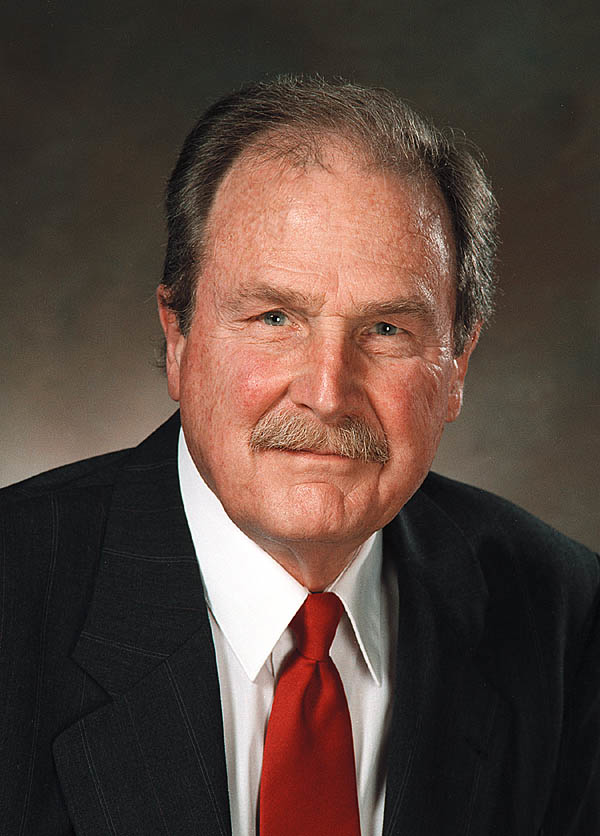
\includegraphics[width=3cm]{5_2}
\begin{center}
\caption{}
\footnotesize{Дэвид Хаффман}
\\\footnotesize{$1925 -- 1999$}
\end{center}
\end{wrapfigure}
Код (алгоритм) Хаффмана был разработан в 1952 году аспирантом Массачусетского технологического института Дэвидом Хаффманом при написании им курсовой работы.
\\Как и алгоритм Шеннона--Фано, основан на частоте повторения. Зная вероятности символов в сообщении, можно описать процедуру построения кодов переменной длины, состоящих из целого количества битов. Символам с большей вероятностью ставятся в соответствие более короткие коды. Коды Хаффмана обладают свойством префиксности, что позволяет однозначно их декодировать.
\\Однако, в отличие от кодов Шеннона--Фано, коды Хаффмана всегда являются оптимальными.
\\Сжатие данных по Хаффману применяется при сжатии фото-- и видеоизображений (JPEG, стандарты сжатия MPEG), в архиваторах (PKZIP, LZH), в протоколах передачи данных MNP5 и MNP7.
\begin{center}
  \textbf{Алгоритм Хаффмана для неоптимальных префиксных кодов}
\end{center}

\begin{enumerate}
  \item Символы входного алфавита образуют список свободных узлов. Каждый узел имеет вес, равный вероятности появления символа в сжимаемом тексте (исходной последовательности). Строится дерево от листьев (узлов) к корню.
  \item Выбираются два свободных узла дерева с наименьшими весами.
  \item Создается их родитель с весом, равным их суммарному весу.
  \item Родитель добавляется в список свободных узлов, а двое его детей удаляются из этого списка.
  \item Одной дуге, выходящей из родителя (узлу с большим весом), ставится в соответствие значение $1$, а другой (узлу с меньшим весом) значение $0$.
  \item Повторяем шаги 2--4, выбирая в качестве одного из свободных узлов родителя, до тех пор, пока в списке свободных узлов не останется только один свободный узел. Он и будет считаться корнем дерева.
  \item Символ входного (первичного) алфавита кодируется последовательностью нулей и единиц в соответствии с распределением их от корня дерева к узлам (листьям).
\end{enumerate}

\emph{\textbf{Пример 1:}}
\\\emph{Задание:} составить код Хаффмана для неоптимальных префиксных кодов для последовательности AAABCCCCCDEEEF. Найти среднюю длину кодового слова.
\\\emph{Решение:} составим список свободных узлов для исходной последовательности:
\\$\bullet$ Символ $A$ с вероятностью $^3/_{14}$;
\\$\bullet$ Символ $B$ с вероятностью $^1/_{14}$;
\\$\bullet$ Символ $C$ с вероятностью $^5/_{14}$;
\\$\bullet$ Символ $D$ с вероятностью $^1/_{14}$;
\\$\bullet$ Символ $E$ с вероятностью $^3/_{14}$;
\\$\bullet$ Символ $F$ с вероятностью $^1/_{14}$.
\\Построим кодовое дерево:
\begin{table}[h]
\centering
\begin{tabular}{c c c c c c}
\multicolumn{6}{l}{DBFAEC ($^1/_{14} + ^1/_{14} + ^1/_{14} + ^3/_{14} + ^3/_{14} + ^5/_{14}$)} \\
$\downarrow$ & \multicolumn{5}{c}{$\downarrow$} \\
C ($^5/_{14}$) & \multicolumn{5}{l}{DBFAE ($^1/_{14} + ^1/_{14} + ^1/_{14} + ^3/_{14} + ^3/_{14}$)} \\
& $\downarrow$ & \multicolumn{4}{c}{$\downarrow$} \\
& E ($^3/_{14}$) & \multicolumn{4}{l}{DBFA ($^1/_{14} + ^1/_{14} + ^1/_{14} + ^3/_{14}$)} \\
& & $\downarrow$ & \multicolumn{3}{c}{$\downarrow$} \\
& & A ($^3/_{14}$) & \multicolumn{3}{l}{DBF ($^1/_{14} + ^1/_{14} + ^1/_{14}$)} \\
& & & $\downarrow$ & \multicolumn{2}{c}{$\downarrow$} \\
& & & F ($^1/_{14}$) & \multicolumn{2}{l}{DB ($^1/_{14} + ^1/_{14}$)} \\
& & & & $\downarrow$ & $\downarrow$ \\
& & & & B ($^1/_{14}$) & D ($^1/_{14}$) \\
\end{tabular}
\end{table}
\\Одной дуге, выходящей из родителя (узлу с большим весом), присвоим значение $1$, а другой (узлу с меньшим весом) -- значение $0$.
\begin{table}[h]
\centering
\begin{tabular}{c c c c c c}
\multicolumn{6}{l}{DBFAEC ($^1/_{14} + ^1/_{14} + ^1/_{14} + ^3/_{14} + ^3/_{14} + ^5/_{14}$)} \\
$\downarrow$ & \multicolumn{5}{l}{$\downarrow$} \\
C ($^5/_{14}$) [0] & \multicolumn{5}{l}{DBFAE ($^1/_{14} + ^1/_{14} + ^1/_{14} + ^3/_{14} + ^3/_{14}$) [1]} \\
& $\downarrow$ & \multicolumn{4}{l}{$\downarrow$} \\
& E ($^3/_{14}$) [0] & \multicolumn{4}{l}{DBFA ($^1/_{14} + ^1/_{14} + ^1/_{14} + ^3/_{14}$) [1]} \\
& & $\downarrow$ & \multicolumn{3}{l}{$\downarrow$} \\
& & A ($^3/_{14}$) [0] & \multicolumn{3}{l}{DBF ($^1/_{14} + ^1/_{14} + ^1/_{14}$) [1]} \\
& & & $\downarrow$ & \multicolumn{2}{l}{$\downarrow$} \\
& & & F ($^1/_{14}$) [0] & \multicolumn{2}{l}{DB ($^1/_{14} + ^1/_{14}$) [1]} \\
& & & & $\downarrow$ & \multicolumn{1}{c}{$\downarrow$} \\
& & & \multicolumn{3}{l}{\qquad B ($^1/_{14}$) [0] \qquad D ($^1/_{14}$) [1]}\\
\end{tabular}
\end{table}
\\
\\
\\Получим следующую таблицу для кодировки:
\\
\begin{table}[h]
\begin{tabular}{|c|c|}
\hline
Символ &  Код \\
\hline
A & 110 \\
B & 11110 \\
C & 0 \\
D & 11111 \\
E & 10 \\
F & 1110 \\
\hline
\end{tabular}
\end{table}
\\Исходная последовательность AAABCCCCCDEEEF кодируется следующей: $110.110.110.11110.0.0.0.0.0.11111.10.10.10.1110$ -- 34 бита.
\\Средняя длина кодового слова: $^5/_{14}\times 1 + ^3/_{14}\times 2 + ^3/_{14}\times 3 + ^1/_{14}\times 4\hm + ^1/_{14}\hm\times 5\hm + ^1/_{14}\hm\times 5\hm = ^{34}/_{14} \approx 2,4.$
\begin{center}
  \textbf{Алгоритм Хаффмана для оптимальных префиксных кодов}
\end{center}

\begin{enumerate}
  \item Символы входного (первичного) алфавита выписывают по убыванию вероятностей (весов) в таблицу.
  \item Выбираются два свободных узла (элемента) с наименьшими весами (вероятностями).
  \item Верхнему узлу (с большим весом) присваивается значение $1$, а нижнему (с меньшим весом) -- $0$.
  \item Создается их родитель с весом, равным их суммарному весу.
  \item Родитель добавляется в список свободных узлов (таблицу), занимая соответствующее место в списке убывающих во величине весов (вероятностей), а двое его детей удаляются из этого списка.
  \item Повторяем шаги 2--5, до тех пор, пока в списке свободных узлов (в таблице) не останется только два свободных узла (элемента).
  \item Символ входного (первичного) алфавита кодируется последовательностью нулей и единиц в соответствии с распределением их от корня к узлам.
\end{enumerate}

\emph{\textbf{Пример 2:}}
\\\emph{Задание:} составить код Хаффмана для неоптимальных префиксных кодов для последовательности AAABCCCCCDEEEF. Найти среднюю длину кодового слова.
\\\emph{Решение:} составим список свободных узлов для исходной последовательности:
\\
\begin{minipage}[h]{\textwidth}
\begin{tabular}{|c|c|}
\hline
Символ &  Вероятность, p \\
\hline
C & $^5/_{14}$ \\
A & $^3/_{14}$ \\
E & $^3/_{14}$ \\
B & $^1/_{14}$ \\
D & $^1/_{14}$ \\
F & $^1/_{14}$ \\
\hline
\end{tabular}
\end{minipage}
\\ \\
\\Построим таблицу:
\\
\\\begin{minipage}[h]{\textwidth}
\begin{tabular}{|c|c||c|c||c|c||c|c||c|c|}
\hline
C & $^5/_{14}$ & C & $^5/_{14}$ & C & $^5/_{14}$ & EDFB & $^6/_{14}$ & CA & $^8/_{14}$ \\
A & $^3/_{14}$ & A & $^3/_{14}$ & A & $^3/_{14}$ & C & $^5/_{14}$ & EDFB & $^6/_{14}$ \\
E & $^3/_{14}$ & E & $^3/_{14}$ & E & $^3/_{14}$ & A & $^3/_{14}$ & & \\
B & $^1/_{14}$ & DF & $^2/_{14}$ & DFB & $^3/_{14}$ & & & &\\
D & $^1/_{14}$ & B & $^1/_{14}$ & & & & & &\\
F & $^1/_{14}$ & & & & & & & &\\
\hline
\end{tabular}
\end{minipage}
\\
\\Верхнему узлу (с большим весом) присвоим значение $1$, а нижнему (с меньшим весом) -- $0$:
\begin{table}[h]
\begin{tabular}{|c|c||c|c||c|c||c|c|}
\hline
C & $^5/_{14}$ & C & $^5/_{14}$ & C & $^5/_{14}$ & EDFB & $^6/_{14}$   \\
A & $^3/_{14}$ & A & $^3/_{14}$ & A & $^3/_{14}$ & C [1] & $^5/_{14}$   \\
E & $^3/_{14}$ & E & $^3/_{14}$ & E [1] & $^3/_{14}$ & A [0] & $^3/_{14}$  \\
B & $^1/_{14}$ & DF [1] & $^2/_{14}$ & DFB [0] & $^3/_{14}$ & & \\
D [1] & $^1/_{14}$ & B [0] & $^1/_{14}$ & & & & \\
F [0] & $^1/_{14}$ & & & & & & \\
\hline
\end{tabular}
\end{table}
\\
\begin{minipage}[h]{6cm}
\begin{tabular}{|c|c|}
\hline
CA [1] & $^8/_{14}$ \\
EDFB [0] & $^6/_{14}$ \\
& \\
& \\
& \\
& \\
\hline
\end{tabular}
\end{minipage}
\\\\\\\\\\\\\\\\\\\\\\
\\Построим кодовое дерево:\\
\\
\begin{minipage}[!h]{\textwidth}
\centering
\begin{tabular}{c c c c c c}
\multicolumn{6}{c}{CAEDFB ($^5/_{14} + ^3/_{14} + ^3/_{14} + ^1/_{14} + ^1/_{14} + ^1/_{14}$)} \\
\multicolumn{2}{c}{$\downarrow$} & \multicolumn{4}{c}{$\downarrow$} \\
\multicolumn{2}{c}{CA ($^5/_{14} + ^3/_{14}$) [1]} & \multicolumn{4}{c}{EDFB ($^3/_{14} + ^1/_{14} + ^1/_{14} + ^1/_{14}$) [0]} \\
$\downarrow$ & $\downarrow$ & \qquad $\downarrow$ & \multicolumn{3}{c}{$\downarrow$} \\
C ($^5/_{14}$) [1] & A ($^3/_{14}$) [0] & E ($^3/_{14}$) [1] & \multicolumn{3}{c}{DFB ($^1/_{14} + ^1/_{14} + ^1/_{14}$) [0]} \\
& & & \multicolumn{2}{c}{$\downarrow$} & $\downarrow$ \\
& & & \multicolumn{2}{r}{DF ($^1/_{14} + ^1/_{14}$) [1]} & B ($^1/_{14}$) [0] \\
\multicolumn{5}{r}{$\downarrow$ \qquad \qquad $\downarrow$ \qquad \qquad} & \\
\multicolumn{5}{r}{D ($^1/_{14}$) [1] \qquad  F ($^1/_{14}$) [0]} & \\
\end{tabular}
\end{minipage}
\\
\\
\\Получим следующую таблицу для кодировки:
\begin{table}[h]
\begin{tabular}{|c|c|}
\hline
Символ &  Код \\
\hline
A & 10 \\
B & 000 \\
C & 11 \\
D & 0011 \\
E & 01 \\
F & 0010 \\
\hline
\end{tabular}
\end{table}
\\Исходная последовательность AAABCCCCCDEEEF кодируется следующей: $10.10.10.000.11.11.11.11.11.0011.01.01.01.0010$ -- 33 бита.
\\Средняя длина кодового слова: $^5/_{14}\times 2 + ^3/_{14}\times 2 + ^3/_{14}\times 2 + ^1/_{14}\times 3\hm + ^1/_{14}\hm\times 4\hm + ^1/_{14}\hm\times 4\hm = ^{33}/_{14} \approx 2,35.$
Классический алгоритм Хаффмана имеет один существенный недостаток. Для восстановления содержимого сжатого текста при декодировании необходимо знать таблицу частот, которую использовали при кодировании. Следовательно, длина сжатого текста увеличивается на длину таблицы частот, которая должна посылаться впереди данных, что может свести на нет все усилия по сжатию данных. Кроме того, необходимость наличия полной частотной статистики перед началом собственно кодирования требует двух проходов по тексту: одного для построения модели текста (таблицы частот и дерева Хаффмана), другого для собственно кодирования.\\

\subsection{Кодирование длин серий}
\emph{\textbf{Кодирование длин серий (кодирование повторов)}} -- алгоритм сжатия данных, заменяющий повторяющиеся символы (серии) на один символ и число его повторов. \emph{\textbf{Серией}} называется последовательность, состоящая из нескольких одинаковых символов. При кодировании (упаковке, сжатии) строка одинаковых символов, составляющих серию, заменяется строкой, содержащей сам повторяющийся символ и количество его повторов.
\\Кодирование длин серий активно применяется при сжатии графических изображений, таких как иконки или графические изображения.
\\
\\\emph{\textbf{Пример :}}
\\\emph{Задание:} применить кодирование длин серий для последовательности \\$AAAAABAAAAABBBBBAAAAA$.
\\\emph{Решение:} посчитаем количество повторяющихся символов:
\\$1.$ $5$ символов $A$;
\\$2.$ $1$ символ $B$;
\\$3.$ $5$ символов $A$;
\\$4.$ $5$ символов $B$;
\\$5.$ $5$ символов $A$.
\\Итого, найдено 5 серий. Заменим серии на число повторов и сам повторяющийся символ: $5A1B5A5B5A$. Получилась последовательность из 10 символов. Исходная последовательность состояла из 21 символа.
\\Коэффициент сжатия: $\frac{21}{10} = 2,1$.

\subsection{Метод относительного кодирования}
В некоторых случаях информация может состоять из блоков данных, каждый из которых может немного отличаться от предыдущего. Примером могут служить последовательные кадры видеоизображения. Для таких случаев используется метод относительного кодирования. Данный подход предполагает запись отличий, существующих между последовательными блоками данных, вместо записи самих этих блоков, т.е. каждый блок кодируется с точки зрения его взаимосвязи с предыдущим блоком. 
\\\emph{\textbf{Пример :}}
\\\emph{Задание:} применить метод относительного кодирования для последовательности чисел \\$1476; 1473; 1480; 1477$.
\\\emph{Решение:} Берем изначально число 1476, смещение до 1473 относительно него равно -3, смещение до 1480 относительно второго числа равно +7; т.о. представим последовательность в следующем виде: 1476; -3; +7; -3.

\subsection{Частотно--зависимое кодирование}
Этот метод сжатия данных предполагает применение частотно--зависимого кодирования, при котором длина битовой комбинации, представляющей элемент данных, обратно пропорциональна частоте использования этого элемента. Такие коды входят в группу кодов переменной длины, т.е. элементы данных в этих кодах представляются битовыми комбинациями различной длины. Если взять английский текст, закодированный с помощью частотно--зависимого метода, то чаще всего встречающиеся символы [e, t, a, i] будут представлены короткими битовыми комбинациями, а те знаки, которые встречаются реже [z, q, x], -- более длинными битовыми комбинациями. В результате мы получим более короткое представление всего текста, чем при использовании обычного кода, подобного Unicode или ASCII. Построение алгоритма, который обычно используется при разработке частотно--зависимых кодов, приписывают Девиду Хаффмануу, поэтому такие коды часто называют кодами Хаффмана.\\
\\\emph{\textbf{Пример :}}
\\\emph{Задание:} требуется закодировать частотно--зависимым методом последовательность:\\ $$\alpha\gamma\alpha\alpha\beta\alpha\alpha\gamma\alpha\alpha\beta\alpha\lambda\alpha\alpha\beta\alpha\beta\alpha\beta\alpha\beta\alpha\alpha,$$
\\\emph{Решение:} последовательность состоит из четырех символов $\alpha, \beta, \gamma$ и $\lambda$. Причем в ней $\alpha$ встречается 15 раз, $\beta$ -- 6 раз, $\gamma$ -- 2 раза и $\lambda$ -- 1 раз.\\
Выберем в соответствии с методом Хаффмана следующий двоичный код для представления символов:\\
\\$\alpha -- 1$
\\$\beta -- 01$
\\$\gamma -- 001$
\\$\lambda -- 000$\\
\\Получим в итоге последовательность: 100111011100111011000110110110110111.
\subsection{Метод Лемпеля--Зива}
Данный метод назван в честь его создателей, Абрахама Лемпеля и Джекоба Зива. Системы кодирования по методу Лемпеля--Зива используют технологию кодирования с применением адаптивного словаря, эта система используется при создании сжатых файлов, называемых zip – файлами. В текущем контексте словарем является набор стандартных блоков,  из которых построено сообщение, которое нужно сжать. Если бы мы хотели сжать текст на английском алфавите, то такими стандартными блоками были бы буквы алфавита. Если бы мы хотели сжать уже закодированные данные, то стандартными блоками были бы цифры 0 и 1. При адаптивном кодировании словарь может изменяться в процессе кодирования.\\
\\В качестве примера рассмотрим алгоритм \textbf{LZ77} – частный случай алгоритма Лемпеля--Зива.\\
Начнем с простого цитирования начальной части сообщения. Затем представим оставшуюся часть сообщения в виде последовательности троек (содержащих два целых числа, за которыми следует символ из сообщения). Каждая такая тройка описывает, как должна строиться следующая часть сообщения на основе предыдущей. Следовательно, словарь, из которого строится сообщение, состоит из самого сообщения.\\
\\\emph{\textbf{Пример :}}
\\\emph{Задание:} дано сжатое сообщение xyxxyzy(5,4,x), необходимо развернуть сообщение так, чтобы получить исходную последовательность.
\\\emph{Решение:} сообщение xyxxyzy(5,4,x) состоит из начального сегмента xyxxyzy, за которым следует тройка (5,4,x).
Чтобы развернуть оставшуюся часть сообщения, необходимо расшифровать тройку (5,4,x). Первое число тройки показывает, на сколько символов нужно вернуться назад в развернутой цепочке.
$$xy\downarrow xxyzy$$
 Далее нужно добавить в конец развернутой цепочки символы, находящиеся в этой позиции. Второе число показывает, сколько символов нужно добавлять.
$$xy\downarrow \textbf{xxyz}y$$
$$xyxxyzyxxyz$$
В завершение добавляем в конец цепочки последний символ тройки.
$$xyxxyzyxxyzx$$
Для того чтобы сжать сообщение с помощью алгоритма LZ77, сначала переписываем начальный сегмент сообщения, затем в этом сегменте ищем самую длинную цепочку, которая совпадает с оставшейся частью сообщения. К этой цепочке будет относиться первая тройка. 
\subsection{Сжатие изображений}
Растровые изображения представляются обычно 3 байта на один пиксел, это приводит к большим и трудно обрабатываемым файлам растровой графики. Для того, чтобы уменьшить требования к памяти, было разработано много схем сжатия изображений. Одна из них, разработанная компанией CompuServe, называется GIF(Graphic Interchange Format -- формат графического обмена). Этот стандарт сжатия решает проблему, сокращая количество цветов, которые могут быть приписаны пикселу, до 256. Это позволяет представить значение каждого пиксела спомощью одного байта вместо трех. Каждому коду при помощи таблицы (палитры) ставится в соответствие определенное сочетание красного, синего и зеленого цветов. Одному из цветов используется значение «прозрачный», то есть через любой участок изображения, которому присвоен этот цвет, виден фон. Эта возможность и простота формата обусловили его широкое использование в компьютерных играх, где многочисленные изображения перемещаются по экрану.\\
\\Другой стандарт сжатия изображений -- JPEG (разработан Joint Photo-- graphic Experts Group -- объединенной группой экспертов в области фотографии) принят производителями цифровых камер для цифровых фотографий. Стандарт JPEG включает в себя несколько способов представления изображения, у каждого из которых своя задача.\\
\\Когда требуется предельная точность, используется метод «без потерь», при котором хранится различие между соседними пикселами, а не интенсивности пикселов.  Различия можно представить более короткими кодами, чем значения, они записываются с помощью кодов переменной длины\\
\\При использовании этого метода сложно менять размеры изображения, поэтому используется базисный стандарт JPEG, который сокращает размер кода, используя для задания состояния пиксела два параметра – яркость и цвет. Причина разделения состоит в том, что человеческий глаз более чувствителен к изменению яркости, чем к изменению цвета. Базисный формат распределяет изображение на блоки размером четыре пиксела, при этом записывается только средний цвет каждого блока. В окончательном представлении сохраняются все быстрые изменения яркости, но при этом стираются быстрые изменения цвета. Каждый блок из четырех пикселов задается только шестью байтами (4 для яркости и 2 для цвета), а не двенадцатью, как если бы один пиксел задавался тремя байтами.\\
\\Дополнительное пространство экономится при записи изменений яркости и цвета, а не их физических значений. Различия записываются при помощи математического метода, который называется дискретным косинусным преобразованием. Окончательный двоичный код затем сжимается при помощи метода  с кодом переменной длины.\\
\\С помощью базисного стандарта  JPEG можно кодировать высококачественные цветные изображения, используя двоичный код, который занимает примерно в двадцать раз меньше памяти, чем формат «три байта на пиксел», используемый во многих сканерах.
\section{Передача данных}
\emph{\textbf{Передача данных} (обмен данными, цифровая передача, цифровая связь)} -- физический перенос данных (цифрового битового потока) в виде сигналов от точки к точке или от точки к нескольким точкам средствами электросвязи по каналу связи, как правило, для последующей обработки средствами вычислительной техники. Примеры подобных каналов -- медные провода, оптическое волокно, беспроводные каналы связи или запоминающее устройство.\\
\subsection{Классификация}
Передача данных может быть \emph{аналоговой} или \emph{цифровой} (то есть поток двоичных сигналов), а также модулирована посредством аналоговой модуляции, либо посредством цифрового кодирования. \emph{Аналоговая} связь является передачей постоянно меняющегося цифрового сигнала, \emph{цифровая} связь является непрерывной передачей сообщений. Сообщения представляют собой либо последовательность импульсов, означающую линейный код (в полосе пропускания), либо ограничивается набором непрерывно меняющейся формы волны, используя метод цифровой модуляции. Такой способ модуляции и соответствующая ему демодуляция осуществляютсямодемным оборудованием.\\
\\Передаваемые данные могут быть цифровыми сообщениями, идущими из источника данных, например, из компьютера или от клавиатуры. Это может быть и аналоговый сигнал — телефонный звонок или видеосигнал, оцифрованный в битовый поток, используя импульсно--кодирующую модуляцию (Pulse Coding Modulation (PCM)) или более расширенные схемы кодирования источника (аналого--цифровое преобразование и сжатие данных). Кодирование источника и декодирование осуществляется кодеком или кодирующим оборудованием.\\
\\ Ко всему вышеперечисленному, передача данных может быть \emph{последовательной} и \emph{параллельной.} \emph{Последовательная} передача — это последовательность передачи элементов сигнала, представляющих символ или другой объект данных. Цифровая последовательная передача — это последовательная передача данных по одному биту за один промежуток времени, последовательно один за одним по одному коммуникационному каналу или компьютерной шине. Так как это требует меньшей обработки сигнала и при этом меньше вероятность ошибки, чем при \emph{параллельной} передаче, то скорость передачи данных по каждому отдельному пути может быть быстрее. Этот механизм может использоваться на более дальних расстояниях, потому что легко может быть передана контрольная цифра (бит чётности, более детально о котором мы поговорим в следующей главе).\\
\\\emph{Параллельной} передачей называется одновременная передача соответствующих элементов сигнала по двум или большему числу путей. Используя множество электрических проводов можно передавать несколько бит одновременно, что позволяет достичь более высоких скоростей передачи, чем при \emph{последовательной} передаче. Этот метод применяется внутри компьютера, например, во внутренних шинах данных, а иногда и во внешних устройствах, таких, как принтеры. Основной проблемой при этом является «перекос», потому что провода при параллельной передаче имеют немного разные свойства, поэтому некоторые биты могут прибыть раньше других, что может повредить сообщение. Бит чётности может способствовать сокращению ошибок. Тем не менее электрический провод при параллельной передаче данных менее надёжен на больших расстояниях, поскольку передача нарушается с гораздо более высокой вероятностью.
\subsection{Типы каналов связи}
\begin{itemize}
\item \emph{Симплекс} -- связь, при которой информация передаётся только в одном направлении;
\item \emph{Дуплекс} -- режим, при котором передача и прием ведутся устройством одновременно по двум физически разделённым каналам связи (по отдельным проводникам, на двух различных частотах и др., за исключением разделения во времени — поочередной передачи);
\item \emph{Полудуплекс} -- режим, при котором, в отличие от дуплексного, передача ведётся по одному каналу связи в обоих направлениях, но с разделением по времени (в каждый момент времени передача ведётся только в одном направлении);
\item \emph{Точка--точка}(сеть из точки в точку) -- простейший вид компьютерной сети, при котором два компьютера соединяются между собой напрямую через коммуникационное оборудование (просто и дешево, но таким образом соединить можно не более двух компьютеров).
\newpage
\item \emph{Многоточечная:}
\begin{itemize}
\item \emph{Шина};
\item \emph{Кольцо};
\item \emph{Звезда};
\item \emph{Ячеистая топология};
\item \emph{Беспроводная сеть}.
\end{itemize}
\end{itemize}